\documentclass[10pt,journal,compsoc, draftclsnofoot,onecolumn]{IEEEtran}

\usepackage{graphicx}
\usepackage{subcaption}
\usepackage{epstopdf}
\usepackage{amssymb}                                         
\usepackage{amsmath}                                         
\usepackage{amsthm}                                          
\usepackage{alltt}                                           
\usepackage{float}
\usepackage{color}
\usepackage{url}
\usepackage{balance}
\usepackage{enumitem}
\usepackage{pstricks, pst-node}
\usepackage{hyperref}
\usepackage{wrapfig}
\usepackage{listings}
\usepackage[margin=0.75in]{geometry}

\geometry{textheight=8.5in, textwidth=6in}

\newcommand{\cred}[1]{{\color{red}#1}}
\newcommand{\cblue}[1]{{\color{blue}#1}}

\usepackage{fancyvrb}
\usepackage{color}
\usepackage[latin1]{inputenc}


\makeatletter
\def\PY@reset{\let\PY@it=\relax \let\PY@bf=\relax%
    \let\PY@ul=\relax \let\PY@tc=\relax%
    \let\PY@bc=\relax \let\PY@ff=\relax}
\def\PY@tok#1{\csname PY@tok@#1\endcsname}
\def\PY@toks#1+{\ifx\relax#1\empty\else%
    \PY@tok{#1}\expandafter\PY@toks\fi}
\def\PY@do#1{\PY@bc{\PY@tc{\PY@ul{%
    \PY@it{\PY@bf{\PY@ff{#1}}}}}}}
\def\PY#1#2{\PY@reset\PY@toks#1+\relax+\PY@do{#2}}

\expandafter\def\csname PY@tok@gd\endcsname{\def\PY@tc##1{\textcolor[rgb]{0.63,0.00,0.00}{##1}}}
\expandafter\def\csname PY@tok@gu\endcsname{\let\PY@bf=\textbf\def\PY@tc##1{\textcolor[rgb]{0.50,0.00,0.50}{##1}}}
\expandafter\def\csname PY@tok@gt\endcsname{\def\PY@tc##1{\textcolor[rgb]{0.00,0.25,0.82}{##1}}}
\expandafter\def\csname PY@tok@gs\endcsname{\let\PY@bf=\textbf}
\expandafter\def\csname PY@tok@gr\endcsname{\def\PY@tc##1{\textcolor[rgb]{1.00,0.00,0.00}{##1}}}
\expandafter\def\csname PY@tok@cm\endcsname{\let\PY@it=\textit\def\PY@tc##1{\textcolor[rgb]{0.25,0.50,0.50}{##1}}}
\expandafter\def\csname PY@tok@vg\endcsname{\def\PY@tc##1{\textcolor[rgb]{0.10,0.09,0.49}{##1}}}
\expandafter\def\csname PY@tok@m\endcsname{\def\PY@tc##1{\textcolor[rgb]{0.40,0.40,0.40}{##1}}}
\expandafter\def\csname PY@tok@mh\endcsname{\def\PY@tc##1{\textcolor[rgb]{0.40,0.40,0.40}{##1}}}
\expandafter\def\csname PY@tok@go\endcsname{\def\PY@tc##1{\textcolor[rgb]{0.50,0.50,0.50}{##1}}}
\expandafter\def\csname PY@tok@ge\endcsname{\let\PY@it=\textit}
\expandafter\def\csname PY@tok@vc\endcsname{\def\PY@tc##1{\textcolor[rgb]{0.10,0.09,0.49}{##1}}}
\expandafter\def\csname PY@tok@il\endcsname{\def\PY@tc##1{\textcolor[rgb]{0.40,0.40,0.40}{##1}}}
\expandafter\def\csname PY@tok@cs\endcsname{\let\PY@it=\textit\def\PY@tc##1{\textcolor[rgb]{0.25,0.50,0.50}{##1}}}
\expandafter\def\csname PY@tok@cp\endcsname{\def\PY@tc##1{\textcolor[rgb]{0.74,0.48,0.00}{##1}}}
\expandafter\def\csname PY@tok@gi\endcsname{\def\PY@tc##1{\textcolor[rgb]{0.00,0.63,0.00}{##1}}}
\expandafter\def\csname PY@tok@gh\endcsname{\let\PY@bf=\textbf\def\PY@tc##1{\textcolor[rgb]{0.00,0.00,0.50}{##1}}}
\expandafter\def\csname PY@tok@ni\endcsname{\let\PY@bf=\textbf\def\PY@tc##1{\textcolor[rgb]{0.60,0.60,0.60}{##1}}}
\expandafter\def\csname PY@tok@nl\endcsname{\def\PY@tc##1{\textcolor[rgb]{0.63,0.63,0.00}{##1}}}
\expandafter\def\csname PY@tok@nn\endcsname{\let\PY@bf=\textbf\def\PY@tc##1{\textcolor[rgb]{0.00,0.00,1.00}{##1}}}
\expandafter\def\csname PY@tok@no\endcsname{\def\PY@tc##1{\textcolor[rgb]{0.53,0.00,0.00}{##1}}}
\expandafter\def\csname PY@tok@na\endcsname{\def\PY@tc##1{\textcolor[rgb]{0.49,0.56,0.16}{##1}}}
\expandafter\def\csname PY@tok@nb\endcsname{\def\PY@tc##1{\textcolor[rgb]{0.00,0.50,0.00}{##1}}}
\expandafter\def\csname PY@tok@nc\endcsname{\let\PY@bf=\textbf\def\PY@tc##1{\textcolor[rgb]{0.00,0.00,1.00}{##1}}}
\expandafter\def\csname PY@tok@nd\endcsname{\def\PY@tc##1{\textcolor[rgb]{0.67,0.13,1.00}{##1}}}
\expandafter\def\csname PY@tok@ne\endcsname{\let\PY@bf=\textbf\def\PY@tc##1{\textcolor[rgb]{0.82,0.25,0.23}{##1}}}
\expandafter\def\csname PY@tok@nf\endcsname{\def\PY@tc##1{\textcolor[rgb]{0.00,0.00,1.00}{##1}}}
\expandafter\def\csname PY@tok@si\endcsname{\let\PY@bf=\textbf\def\PY@tc##1{\textcolor[rgb]{0.73,0.40,0.53}{##1}}}
\expandafter\def\csname PY@tok@s2\endcsname{\def\PY@tc##1{\textcolor[rgb]{0.73,0.13,0.13}{##1}}}
\expandafter\def\csname PY@tok@vi\endcsname{\def\PY@tc##1{\textcolor[rgb]{0.10,0.09,0.49}{##1}}}
\expandafter\def\csname PY@tok@nt\endcsname{\let\PY@bf=\textbf\def\PY@tc##1{\textcolor[rgb]{0.00,0.50,0.00}{##1}}}
\expandafter\def\csname PY@tok@nv\endcsname{\def\PY@tc##1{\textcolor[rgb]{0.10,0.09,0.49}{##1}}}
\expandafter\def\csname PY@tok@s1\endcsname{\def\PY@tc##1{\textcolor[rgb]{0.73,0.13,0.13}{##1}}}
\expandafter\def\csname PY@tok@sh\endcsname{\def\PY@tc##1{\textcolor[rgb]{0.73,0.13,0.13}{##1}}}
\expandafter\def\csname PY@tok@sc\endcsname{\def\PY@tc##1{\textcolor[rgb]{0.73,0.13,0.13}{##1}}}
\expandafter\def\csname PY@tok@sx\endcsname{\def\PY@tc##1{\textcolor[rgb]{0.00,0.50,0.00}{##1}}}
\expandafter\def\csname PY@tok@bp\endcsname{\def\PY@tc##1{\textcolor[rgb]{0.00,0.50,0.00}{##1}}}
\expandafter\def\csname PY@tok@c1\endcsname{\let\PY@it=\textit\def\PY@tc##1{\textcolor[rgb]{0.25,0.50,0.50}{##1}}}
\expandafter\def\csname PY@tok@kc\endcsname{\let\PY@bf=\textbf\def\PY@tc##1{\textcolor[rgb]{0.00,0.50,0.00}{##1}}}
\expandafter\def\csname PY@tok@c\endcsname{\let\PY@it=\textit\def\PY@tc##1{\textcolor[rgb]{0.25,0.50,0.50}{##1}}}
\expandafter\def\csname PY@tok@mf\endcsname{\def\PY@tc##1{\textcolor[rgb]{0.40,0.40,0.40}{##1}}}
\expandafter\def\csname PY@tok@err\endcsname{\def\PY@bc##1{\setlength{\fboxsep}{0pt}\fcolorbox[rgb]{1.00,0.00,0.00}{1,1,1}{\strut ##1}}}
\expandafter\def\csname PY@tok@kd\endcsname{\let\PY@bf=\textbf\def\PY@tc##1{\textcolor[rgb]{0.00,0.50,0.00}{##1}}}
\expandafter\def\csname PY@tok@ss\endcsname{\def\PY@tc##1{\textcolor[rgb]{0.10,0.09,0.49}{##1}}}
\expandafter\def\csname PY@tok@sr\endcsname{\def\PY@tc##1{\textcolor[rgb]{0.73,0.40,0.53}{##1}}}
\expandafter\def\csname PY@tok@mo\endcsname{\def\PY@tc##1{\textcolor[rgb]{0.40,0.40,0.40}{##1}}}
\expandafter\def\csname PY@tok@kn\endcsname{\let\PY@bf=\textbf\def\PY@tc##1{\textcolor[rgb]{0.00,0.50,0.00}{##1}}}
\expandafter\def\csname PY@tok@mi\endcsname{\def\PY@tc##1{\textcolor[rgb]{0.40,0.40,0.40}{##1}}}
\expandafter\def\csname PY@tok@gp\endcsname{\let\PY@bf=\textbf\def\PY@tc##1{\textcolor[rgb]{0.00,0.00,0.50}{##1}}}
\expandafter\def\csname PY@tok@o\endcsname{\def\PY@tc##1{\textcolor[rgb]{0.40,0.40,0.40}{##1}}}
\expandafter\def\csname PY@tok@kr\endcsname{\let\PY@bf=\textbf\def\PY@tc##1{\textcolor[rgb]{0.00,0.50,0.00}{##1}}}
\expandafter\def\csname PY@tok@s\endcsname{\def\PY@tc##1{\textcolor[rgb]{0.73,0.13,0.13}{##1}}}
\expandafter\def\csname PY@tok@kp\endcsname{\def\PY@tc##1{\textcolor[rgb]{0.00,0.50,0.00}{##1}}}
\expandafter\def\csname PY@tok@w\endcsname{\def\PY@tc##1{\textcolor[rgb]{0.73,0.73,0.73}{##1}}}
\expandafter\def\csname PY@tok@kt\endcsname{\def\PY@tc##1{\textcolor[rgb]{0.69,0.00,0.25}{##1}}}
\expandafter\def\csname PY@tok@ow\endcsname{\let\PY@bf=\textbf\def\PY@tc##1{\textcolor[rgb]{0.67,0.13,1.00}{##1}}}
\expandafter\def\csname PY@tok@sb\endcsname{\def\PY@tc##1{\textcolor[rgb]{0.73,0.13,0.13}{##1}}}
\expandafter\def\csname PY@tok@k\endcsname{\let\PY@bf=\textbf\def\PY@tc##1{\textcolor[rgb]{0.00,0.50,0.00}{##1}}}
\expandafter\def\csname PY@tok@se\endcsname{\let\PY@bf=\textbf\def\PY@tc##1{\textcolor[rgb]{0.73,0.40,0.13}{##1}}}
\expandafter\def\csname PY@tok@sd\endcsname{\let\PY@it=\textit\def\PY@tc##1{\textcolor[rgb]{0.73,0.13,0.13}{##1}}}

\def\PYZbs{\char`\\}
\def\PYZus{\char`\_}
\def\PYZob{\char`\{}
\def\PYZcb{\char`\}}
\def\PYZca{\char`\^}
\def\PYZam{\char`\&}
\def\PYZlt{\char`\<}
\def\PYZgt{\char`\>}
\def\PYZsh{\char`\#}
\def\PYZpc{\char`\%}
\def\PYZdl{\char`\$}
\def\PYZti{\char`\~}
% for compatibility with earlier versions
\def\PYZat{@}
\def\PYZlb{[}
\def\PYZrb{]}
\makeatother


\begin{document}

\title{
Progress Report\\
3D Object Pose Tracking for Robotics Grasping\\
CS462 Winter 2019
}
\author{Connor Campbell, Chase McWhirt and Jiawei Mo}

\maketitle

\begin{abstract}
Despite a serious delay (not receiving data) out of our group's control, we have been making steady progress overall.
We have created masks for twenty one of the 2,800 images provided to us during week six.
From these, were able to build a Python script and execute a k-means clustering to generate a mask automatically. 
In the future, we have three more methods to implement, one of which will be an upgraded k-means clustering.
\end{abstract}

\IEEEdisplaynontitleabstractindextext
\IEEEpeerreviewmaketitle

\newpage
\pagebreak
\tableofcontents
\pagebreak

\section{Purpose and Goals}
The goal of this project is to use computer vision to accurately identify a robot arm.
Our aim is 80-90\% accuracy with false negatives being more acceptable than false positives.
Our method has to be fast enough to run in real time as its input will be a video stream.
We are attempting four different methods to see which one works best and will submit the best option, even if it fails to meet our accuracy goals.

\noindent
\section{Progress}
Due to a serious delay, we were unable to begin working on this project until we received images of the robot arm during week 6.
Even after that, we were on unable to implement methods that required nearest neighbor groupings until week 8.
However, despite the short amount of time, for the beta, we've implemented a functionally completed K-means script, a basic support vector machine script, a custom neural network (still working towards a completed basic implementation), and some data processing scripts.

\subsection{Support Vector Machine}
For beta level functionality, the support vector machine has been implemented on a basic level.
It still needs to incorporate nearest neighbor groupings and possibly use a different setup.
However, when given an input directory and an output directory, it can create masks based on input images.

\subsection{Supporting Data Processing Scripts}
There are two main supporting scripts.
The first analyzes a two masks and outputs the differences.
The differences can be true positives or negatives, or false positives or negatives.
The more true positives and negatives, the more accurately the implemented mask was created.
The second supporting script simulates a specification change in which we'll only be checking part of the image with arm and ignoring the rest.

\section{Remaining Work}
Of the three implementations, the custom neural network needs a completed basic implementation.
The support vector machine will require nearest neighbor incorporation and a much more intensively trained model.
K-means also requires nearest neighbor incorporation as well as some quality of life changes.

\section{Obstacles and Solutions}
\subsection{Waiting Data}
We did not receive the necessary data (2800 frames of video separated for us) for nearly six weeks. That is not including the fact that we were expecting to get data near the end of last term, not near the beginning of the term, let alone the over half way through the term we actually ended up waiting. There was no way for us to solve this problem on our own--the data had to come from our client.

\subsection{Accuracy}
When the image set was received and the sample images were labeled, we started to implement K-means algorithm to divide pixels into different clusters. The early trials showed a low accuracy since we labeled the image by only two colors. Two clusters, which were white and black pixels, resulted in the program not being able to identify complicated color chromatic aberration. The created mask labeled part of the robotic arm as white pixels and also marked other pixels white, including cables and stands, which led to a low accuracy labeling. \\

\noindent To improve created masks labeling accuracy, we incremented the number of clusters to 4. Since the image was supported by RGB values, each pixel would have $4^3$ probabilities of the color. Then, by checking each pixel on the created masks and labeled masks at the robotic arm position, we could manually assign the RGB value to certain pixel. In this program, we assigned white color to the robotic arm and left the other things black.
\\

\noindent Furthermore, another test model based on HSV color space system has been implemented. Similar to previous RGB base model, it also set 4 to the cluster number. The point is that the HSV values will generate a different mask. The following shows the visualized masks based on RGB and HSV.

\begin{figure}[H]
  \begin{center}
    \includegraphics[width=0.7\textwidth]{hsv_test_4.png}
  \end{center}
  \caption{A sample of created masks based on HSV. Number of clusters is 4.}
\end{figure}

\begin{figure}[H]
  \begin{center}
    \includegraphics[width=0.7\textwidth]{test.png}
  \end{center}
  \caption{A sample of created masks based on RGB. Number of clusters is 4.}
\end{figure}

\noindent From Fig. 1 and Fig. 2, there is an apparent difference between HSV and RGB models. By zooming in the arm areas of two visualized masks, it indicates that the RGB model has a better performance of distinguished and colored pixels. For an instance, the light pink pixels around the arm fingers, in Fig. 1, highlights that the HSV model would assign ambiguous boundary for different clusters. Therefore, we chose RGB based model to assign white and black color to related pixels. 

\subsection{Neural Network}
For the custom neural network implementation, the Fast Artificial Neural Network (FANN) library was used. The algorithms for reading an image for training the network, then implementing the network over an image is in place, but there are a few problems. For one, the FANN library wants to run on a different architecture than the default version of OpenCV (FANN wants to be built on an x86 platform, while OpenCV wants x64). As a result, the functions that use these need to be on separate executables that communicate through files. Connor intends to fix this over Spring Break, e.  

\subsection{Support Vector Machine}
The current main issue with the support vector machine is training it.
When given a single 640x480 image, training the model can take four to five hours.
There is no clear way to optimize this so that it can run more quickly.
Though, some attempts will made over Spring break.
Next, it also needs to run with knowledge of nearest neighbors.
That too will be implemented over Spring break.

\section{Part of Code}
\subsection{Store Images}
We used Numpy to store the images in a four dimensional matrix. The first dimension is the index of the picture. The second is the height of the image and width locates at the third dimension. The RGB values were stored at the last position. The following is the code to store images in program memory.

\begin{lstlisting}
def read_img(path, if_gscale):
    i = 0
    for filename in os.listdir(path):
        i += 1
        print(filename)
        hand = mpimg.imread(path + filename)
        if if_gscale:
            hand = greyscale(hand)
        else:
            hand = hand[...,:3]
        if i == 1:
            set = np.array(hand)
        else:  
            set = np.concatenate( ( set, np.array(hand) ), axis = 0 )

    if if_gscale:
        set = set.reshape( i, 480, 640)
    else:
        set = set.reshape( i, 480, 640, 3)
    print(path, 'set shape = ', set.shape)

    return set
\end{lstlisting}

\subsection{Flatten Matrix}
Moreover, it is important to flatten the high dimensional matrix as a one dimension array structure. The reason is that the K-means algorithm can only work on the one dimension or two dimension data structure. The process of jpeg.reshape below will return a one dimension array and every single element represents a pixel value. It can be arbitrary value of RGB. 

\begin{lstlisting}
jpeg_feed = jpeg.reshape(jpeg.shape[0] * jpeg.shape[1] * jpeg.shape[2] * jpeg.shape[3], 1)
\end{lstlisting}

\subsection{Predict}
The main process of K-means algorithm is to create a mask of the original data. By setting number of clusters and predicting the images, we received the mask stored in the variable, result. Its elements were integers from 0 to 3. After reshaping it to image matrix, we could show this mask and save it to the driver. 

\begin{lstlisting}
n_clusters = 4
kmeans = KMeans(n_clusters=n_clusters, random_state=0).fit(jpeg_feed)
result = kmeans.predict(jpeg_feed)
result = result.reshape(21, 480, 640, 3)
\end{lstlisting}

\section{Alpha Build}
Below is a demonstration of our straw man method using K-mean clustering. We took 21 images from the data set and used Photoshop to create masks of the arm by hand. We used these as training data to define clusters of pixel to recognize as being part of the hand based on color. It does a decent job of recognizing the parts of the arm over the brown table, but gets confused on the side of the image. \\

\noindent This reason why the program fails to recognize the side is that the K-means algorithm assigns same value to some of the side part and the robotic arm. Thus, by changing the arm color to white, the side part will also turn to white. The base can be easily separated from arm because it has similar and grouped colors. However, the robotic arm has detailed components and their colors are close to the cable color and stand color, which is hard for K-means to recognize.

\begin{figure}[H]
  \begin{center}
    \includegraphics[width=0.7\textwidth]{original.jpeg}
  \end{center}
  \caption{An image of the robot arm from the data set.}
\end{figure}

\begin{figure}[H]
 \begin{center}
    \includegraphics[width=0.7\textwidth]{photoshop.png}
 \end{center}
 \caption{A mask made by hand with Photoshop.}
\end{figure}


\begin{figure}[H]
  \begin{center}
    \includegraphics[width=0.7\textwidth]{kmeans.png}
  \end{center}
  \caption{A sample mask generated with the straw man (K-means) method.}
\end{figure}

\noindent According to Fig. 5, the outline of the robotics arm was recognized successfully. Notice that there exists a wide white boundary. However, the information in side areas are not considered. Then we added a new feature which is to assign a suitable rectangle around the arm and store the rectangle coordinates into a .csv file. During the masks creation process, program reads the .csv file and then uses the coordinates to paint black on each pixel that is not in the marked rectangle. Fig. 6 will illustrate this methods. 

\begin{figure}[H]
  \begin{center}
    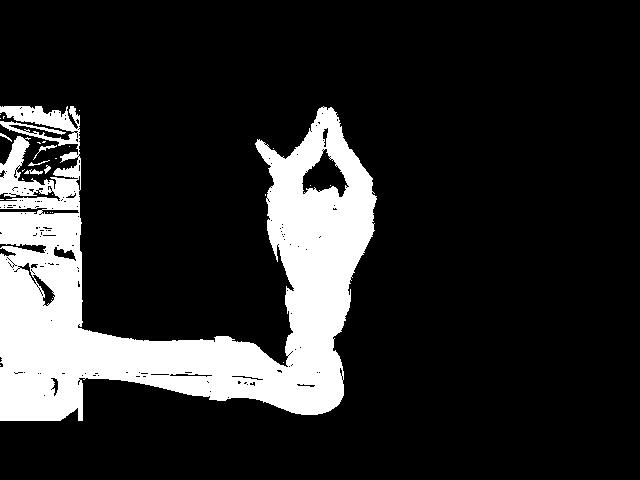
\includegraphics[width=0.7\textwidth]{test_7.png}
  \end{center}
  \caption{A sample mask generated with the straw man (K-means) method plus rectangle process.}
\end{figure}


\section{Next Steps}
In our most recent meeting with our sponsor, we have decided to change our approach to the last three implementations.
Originally, we were going to have another piece of data.
This would have been a file with all of the arm poses associated with the 2,800 images, which are frames of video, we were given.
Instead, we are now using the timestamp of each frame within the video.
Unfortunately, this will likely prove to be ineffective in practice as we won't have a nearest neighbor parser that can run in real time which could have significantly boosted accuracy.
Despite this, we'll implement a k-means clustering method with nearest neighbor and try to optimize the combination.
It's possible that there won't be any improvement.
The last two implementations need more work in order to be fully completed.
We've also received some specification changes for our implementation with K-means which has been implemented.


\end{document}